\documentclass[12pt,a4paper]{article}
\usepackage[utf8]{inputenc}
\usepackage{amsmath}
\usepackage{amssymb}
\usepackage{graphicx}
\usepackage{tikz}
\usepackage{booktabs}
\usepackage{float}
\usepackage{hyperref}
\usepackage{enumitem}
\usepackage[margin=2.5cm]{geometry}
\usepackage{titlesec}
\usepackage{xcolor}
\usepackage{mdframed}
\usepackage{longtable}
\usepackage{placeins}
\usepackage{cleveref}
\usepackage{algorithm}
\usepackage{algpseudocode}
\usepackage{tikz}
\usetikzlibrary{shapes,arrows,positioning,shapes.geometric}

% Define modern colors
\definecolor{definitionheader}{RGB}{41, 128, 185} % Blue
\definecolor{explanationheader}{RGB}{46, 204, 113} % Green
\definecolor{observationheader}{RGB}{230, 126, 34} % Orange
\definecolor{boxbg}{RGB}{248, 249, 250} % Light gray background

% Style configurations
\titleformat{\section}
{\normalfont\LARGE\bfseries}{\thesection}{1em}{}[\vspace{0.2cm}]
\titleformat{\subsection}
{\normalfont\Large\bfseries}{\thesubsection}{1em}{}[\vspace{0.1cm}]

% Modern box styles
\mdfdefinestyle{definitionstyle}{
    linecolor=definitionheader,
    backgroundcolor=boxbg,
    linewidth=0.5pt,
    roundcorner=5pt,
    innertopmargin=10pt,
    innerbottommargin=10pt,
    innerleftmargin=12pt,
    innerrightmargin=12pt,
    skipabove=\baselineskip,
    skipbelow=\baselineskip,
    needspace=3\baselineskip,
    frametitlebackgroundcolor=definitionheader,
    frametitlefont=\normalfont\bfseries\color{white},
    frametitlerule=true,
    frametitleaboveskip=3pt,
    frametitlebelowskip=7pt,
    frametitlerulewidth=0pt
}

\mdfdefinestyle{explanationstyle}{
    linecolor=explanationheader,
    backgroundcolor=boxbg,
    linewidth=0.5pt,
    roundcorner=5pt,
    innertopmargin=10pt,
    innerbottommargin=10pt,
    innerleftmargin=12pt,
    innerrightmargin=12pt,
    skipabove=\baselineskip,
    skipbelow=\baselineskip,
    needspace=3\baselineskip,
    frametitlebackgroundcolor=explanationheader,
    frametitlefont=\normalfont\bfseries\color{white},
    frametitlerule=true,
    frametitleaboveskip=3pt,
    frametitlebelowskip=7pt,
    frametitlerulewidth=0pt
}

\mdfdefinestyle{observationstyle}{
    linecolor=observationheader,
    backgroundcolor=boxbg,
    linewidth=0.5pt,
    roundcorner=5pt,
    innertopmargin=10pt,
    innerbottommargin=10pt,
    innerleftmargin=12pt,
    innerrightmargin=12pt,
    skipabove=\baselineskip,
    skipbelow=\baselineskip,
    needspace=3\baselineskip,
    frametitlebackgroundcolor=observationheader,
    frametitlefont=\normalfont\bfseries\color{white},
    frametitlerule=true,
    frametitleaboveskip=3pt,
    frametitlebelowskip=7pt,
    frametitlerulewidth=0pt
}

% Custom environments with modern headers
\newenvironment{definition}[1]
{\begin{mdframed}[style=definitionstyle,frametitle={Definition: #1}]}
{\end{mdframed}}

\newenvironment{explanation}
{\begin{mdframed}[style=explanationstyle,frametitle={Explanation}]}
{\end{mdframed}}

\newenvironment{observation}
{\begin{mdframed}[style=observationstyle,frametitle={Observation}]}
{\end{mdframed}}

% Hyperref configuration
\hypersetup{
    colorlinks=true,
    linkcolor=black,
    filecolor=black,
    urlcolor=blue,
    citecolor=black
}

% List styling
\setlist[itemize]{leftmargin=*,label=\textbullet,itemsep=0.2em,parsep=0.2em}

\title{\textbf{\LARGE Service Delivery Models:\\[0.3em] Formal Definitions and Analysis Framework}}
\author{\Large}
\date{\today}

\begin{document}

\maketitle
\thispagestyle{empty}
\tableofcontents
\clearpage

\section{Introduction}
This document outlines a practical framework for evaluating and implementing different service delivery models. It provides concrete formulas, metrics, and decision criteria to help teams analyze costs and benefits of various delivery approaches. 

\subsection{Purpose and Scope}
\begin{definition}{Framework Purpose}
The framework serves several key purposes:
\begin{itemize}
    \item Standardize the evaluation of service delivery options
    \item Provide quantitative methods for cost-benefit analysis
    \item Enable data-driven decision making
    \item Account for both direct and indirect costs
    \item Consider quality and efficiency impacts
\end{itemize}
\end{definition}

\begin{explanation}
The analysis framework is built around two fundamental models:
\begin{itemize}
    \item \textbf{Team-Based Model:} Focuses on dedicated service teams
    \item \textbf{Ticket-Based Model:} Centers on service requests
    \item \textbf{Transformation Options:}
    \begin{itemize}
        \item Platform Automation
        \item Outsourcing
        \item Hybrid Solutions
    \end{itemize}
\end{itemize}
\end{explanation}

\subsection{Model Overview}

\begin{explanation}
The analysis framework is built around two fundamental models, each representing a different approach to measuring and managing service delivery:

\textbf{Team-Based Model:} Focuses on the costs and efficiency of dedicated service teams, measuring productivity in terms of time and resource utilization.

\textbf{Ticket-Based Model:} Centers on individual service requests, measuring efficiency in terms of resolution times and throughput.

Each model can be transformed through three strategic approaches:
\begin{itemize}
    \item \textbf{Platform Automation:} Investment in technology to automate processes
    \item \textbf{Outsourcing:} Transfer of operations to external providers
    \item \textbf{Hybrid:} Combination of automation and outsourcing
\end{itemize}
\end{explanation}

\section{Common Variables and Constants}
\subsection{Time Variables}

Time-based calculations are fundamental to service delivery analysis, as they directly impact costs, efficiency, and resource utilization. The following variables provide a standardized approach to temporal measurements.

\begin{definition}{Time Parameters}
\begin{align*}
    T_{month} &= 160 \text{ hours} & T_{year} &= 1920 \text{ hours} \\
    t &= \text{Time period} & \Delta t &= 36 \text{ months}
\end{align*}
\end{definition}

\begin{explanation}
\textbf{Standard Month:}
\begin{itemize}
    \item 40-hour work weeks
    \item 4 weeks per month
    \item Excludes holidays/leave
\end{itemize}
\textbf{Analysis Horizon:}
\begin{itemize}
    \item Implementation phase
    \item Stabilization phase
    \item Benefits realization
\end{itemize}
\end{explanation}

\subsection{Financial Variables}
These variables capture both direct costs and the time value of money, enabling comprehensive financial evaluation.

\begin{definition}{Financial Parameters}
Core financial metrics:
\begin{align*}
    r &= \text{Discount rate} & NPV &= \text{Net Present Value} \\
    i &= \text{Inflation rate} & ROI &= \text{Return on Investment} \\
    IRR &= \text{Internal Rate of Return} & &
\end{align*}
\end{definition}

\begin{explanation}
\textbf{Key Applications:}
\begin{itemize}
    \item Time value calculations
    \item Investment analysis
    \item Cost comparisons
    \item Risk adjustments
\end{itemize}
\textbf{Discount Rate Components:}
\begin{itemize}
    \item Cost of capital
    \item Risk premium
    \item Market conditions
\end{itemize}
\end{explanation}

\section{Team-Based Model}
The team-based model represents a traditional approach to service delivery, where dedicated teams handle various service requests and operational tasks.

\subsection{Base Case Analysis}
The base case establishes the current state of operations, serving as a reference point for comparing different transformation options. It captures all relevant costs and efficiency metrics of the existing team-based delivery model.

\begin{definition}{Team Model Variables}
Let $\mathcal{T}$ represent the team-based model:
\begin{align*}
    n &= \text{Team size (FTEs)} & h &= \text{Hourly rate} \\
    \eta_s &= \text{Service efficiency} & \eta_o &= \text{Operational overhead} \\
    w &= \text{Working hours/month} & &
\end{align*}
\end{definition}

\begin{explanation}
\textbf{Model Components:}
\begin{itemize}
    \item FTEs: Dedicated team members
    \item Efficiency: Productive time ratio
    \item Overhead: Management costs
    \item Hours: Service delivery time
\end{itemize}
\end{explanation}

\subsection{Base Cost Structure}
The following formulation provides a comprehensive view of all cost components in the current delivery model.

\begin{definition}{Base Team Cost}
Monthly base cost calculation:
\begin{equation}
    C_b = n \cdot h \cdot w \cdot \eta_s \cdot (1 + \eta_o)
\end{equation}
\textbf{Components:}
\begin{itemize}
    \item $n \cdot h \cdot w$: Labor cost
    \item $\eta_s$: Efficiency factor
    \item $(1 + \eta_o)$: Overhead factor
\end{itemize}
\end{definition}

\begin{explanation}
\textbf{Cost Factors:}
\begin{itemize}
    \item Direct labor costs
    \item Service efficiency impact
    \item Operational overhead
\end{itemize}
\textbf{Benefits:}
\begin{itemize}
    \item Clear cost structure
    \item Efficiency tracking
    \item Resource optimization
\end{itemize}
\end{explanation}

\subsection{Platform Solution}
Platform automation represents a transformative approach to service delivery. This solution requires upfront investment but can deliver long-term benefits through improved efficiency and scalability.

\begin{definition}{Platform Variables}
For solution $\mathcal{P}$:
\begin{align*}
    P_i &= \text{Initial investment} & P_m &= \text{Monthly maintenance} \\
    \alpha_t &= \text{Team reduction} \in [0,1] & \alpha_p &= \text{Process efficiency} \in [0,1] \\
    T_i &= \text{Implementation time} & &
\end{align*}
\end{definition}

\begin{explanation}
\textbf{Key Elements:}
\begin{itemize}
    \item Investment: Development and setup costs
    \item Maintenance: Ongoing platform costs
    \item Team Reduction: Automated task replacement
    \item Process Efficiency: Streamlined operations
    \item Timeline: Implementation and rollout
\end{itemize}
\end{explanation}

\subsubsection{Platform Cost Structure}
The platform cost structure reflects both the initial investment and ongoing operational costs.

\begin{definition}{Platform Cost}
Monthly cost after implementation:
\begin{equation}
    C_p = C_b \cdot (1 - \alpha_t) \cdot (1 - \alpha_p) + P_m
\end{equation}
\textbf{Impact Factors:}
\begin{itemize}
    \item Team size reduction through automation
    \item Process efficiency improvements
    \item Ongoing maintenance requirements
\end{itemize}
\end{definition}

\begin{observation}
\textbf{Cost Benefits:}
\begin{itemize}
    \item Reduced labor requirements
    \item Improved process efficiency
    \item Standardized operations
\end{itemize}
\textbf{Key Considerations:}
\begin{itemize}
    \item Initial investment planning
    \item Maintenance cost management
    \item Training and transition needs
\end{itemize}
\end{observation}

\subsection{Outsourcing Solution}
Outsourcing presents an alternative transformation path, transferring service delivery responsibilities to external providers. While this approach can offer immediate cost benefits, it introduces various challenges and risks that must be evaluated.

\begin{definition}{Outsourcing Variables}
For solution $\mathcal{O}$:
\begin{align*}
    v &= \text{Vendor hourly rate} & \beta_m &= \text{Management overhead} \in [0,1] \\
    \beta_q &= \text{Quality impact} \in [0,1] & \beta_k &= \text{Knowledge loss} \in [0,1] \\
    O_t &= \text{Transition cost} & T_t &= \text{Transition time}
\end{align*}
\end{definition}

\begin{explanation}
\textbf{Impact Areas:}
\begin{itemize}
    \item Vendor Management: Coordination and oversight
    \item Service Quality: Performance standards
    \item Knowledge Retention: Critical information
    \item Transition Process: Implementation steps
\end{itemize}
\textbf{Risk Factors:}
\begin{itemize}
    \item Quality degradation over time
    \item Knowledge transfer challenges
    \item Management overhead increase
    \item Transition period disruption
\end{itemize}
\end{explanation}

\subsubsection{Outsourcing Cost Structure}
The outsourcing cost structure must account for both direct vendor costs and various indirect impacts on service delivery. This view ensures all relevant factors are considered.

\begin{definition}{Outsourcing Cost}
Monthly cost calculation:
\begin{equation}
    C_o = v \cdot w \cdot n \cdot (1 + \beta_m) \cdot (1 + \beta_q) \cdot (1 + \beta_k \cdot \log_{10}(T_t + 1))
\end{equation}
\textbf{Cost Components:}
\begin{itemize}
    \item Base: $v \cdot w \cdot n$
    \item Management: $(1 + \beta_m)$
    \item Quality: $(1 + \beta_q)$
    \item Knowledge: $1 + \beta_k \cdot \log_{10}(T_t + 1)$
\end{itemize}
\end{definition}

\begin{observation}
\textbf{Time Impact:}
\begin{itemize}
    \item Initial knowledge transfer challenges
    \item Gradual process stabilization
    \item Long-term expertise erosion
\end{itemize}
\textbf{Quality Factors:}
\begin{itemize}
    \item Service level maintenance
    \item Process standardization
    \item Knowledge documentation
\end{itemize}
\end{observation}

\subsection{Hybrid Solution Variables}
The hybrid approach combines elements of both platform automation and outsourcing.

\begin{definition}{Hybrid Variables}
For the hybrid solution $\mathcal{H}$:
\begin{align*}
    \gamma_p &= \text{Platform portion} \in [0,1] \\
    \gamma_o &= \text{Outsourced portion} \in [0,1] \\
    P_h &= \text{Reduced platform investment} \\
    v_h &= \text{Negotiated vendor rate}
\end{align*}
where $\gamma_p + \gamma_o \leq 1$
\end{definition}

\begin{explanation}
The hybrid approach combines platform and outsourcing benefits:
\begin{itemize}
    \item Balanced workload distribution
    \item Reduced platform investment needs
    \item Potentially lower vendor rates
    \item Flexibility in service delivery
\end{itemize}

Key considerations include:
\begin{itemize}
    \item Optimal work distribution
    \item Integration requirements
    \item Coordination overhead
    \item Risk diversification
\end{itemize}
\end{explanation}

\section{Ticket-Based Model}
The ticket-based model focuses on individual service requests as the primary unit of analysis. This approach is well-suited for organizations with clearly defined service requests, standardized processes, and measurable resolution times. It provides a granular view of service delivery costs and efficiency.

\subsection{Base Case Analysis}
The base case for the ticket-based model establishes current performance metrics and costs associated with handling individual service requests. This analysis provides insights into volume patterns, resource requirements, and efficiency opportunities.

\begin{definition}{Ticket Model Variables}
Let $\mathcal{B}$ represent the ticket-based model with:
\begin{align*}
    m &= \text{Monthly tickets} \\
    t_h &= \text{Hours per ticket} \\
    p &= \text{People per ticket} \\
    h &= \text{Hourly rate} \\
    \sigma &= \text{SLA compliance rate} \in [0,1]
\end{align*}
\end{definition}

\begin{explanation}
The ticket-based model focuses on individual service requests:
\begin{itemize}
    \item Volume-based measurement
    \item Resource requirements per ticket
    \item Service level compliance
    \item Direct cost attribution
\end{itemize}

This approach is particularly suitable for:
\begin{itemize}
    \item Help desk operations
    \item Service request handling
    \item Incident management
    \item Standard service delivery
\end{itemize}
\end{explanation}

\subsection{Ticket Cost Structure}

\begin{definition}{Base Ticket Cost}
The monthly base ticket cost $C_t$ is:
\begin{equation}
    C_t = m \cdot t_h \cdot p \cdot h
\end{equation}
\end{definition}

\begin{explanation}
The base ticket cost incorporates:
\begin{itemize}
    \item Volume of service requests
    \item Time investment per request
    \item Required staff involvement
    \item Labor cost rates
\end{itemize}

This formula enables:
\begin{itemize}
    \item Per-ticket cost analysis
    \item Volume-based planning
    \item Resource allocation optimization
    \item Service level management
\end{itemize}
\end{explanation}

\subsection{Outsourcing Impact on Ticket-Based Model}
\begin{definition}{Ticket Outsourcing Variables}
For the ticket-based outsourcing model $\mathcal{TO}$:
\begin{align*}
    v_t &= \text{Vendor cost per ticket} \\
    \mu &= \text{Ticket multiplication factor} \geq 1 \\
    \tau &= \text{Resolution time factor} \geq 1 \\
    \omega &= \text{Rework probability} \in [0,1] \\
    \theta &= \text{Quality threshold} \in [0,1]
\end{align*}
\end{definition}

\begin{explanation}
The ticket-based outsourcing model introduces quality impact through:
\begin{itemize}
    \item Ticket multiplication ($\mu$): Additional tickets generated due to incomplete or incorrect resolutions
    \item Extended resolution times ($\tau$): Increased handling time due to communication overhead
    \item Rework probability ($\omega$): Likelihood of ticket reopening
    \item Quality threshold ($\theta$): Minimum acceptable resolution quality
\end{itemize}
\end{explanation}

\begin{definition}{Outsourced Ticket Cost}
The effective monthly outsourced ticket cost $C_{to}$ is:
\begin{equation}
    C_{to} = m \cdot v_t \cdot \mu \cdot (1 + \omega) \cdot \tau
\end{equation}

The effective number of tickets handled becomes:
\begin{equation}
    m_{eff} = m \cdot \mu \cdot (1 + \omega)
\end{equation}
\end{definition}

\begin{observation}
Quality degradation in ticket-based outsourcing manifests through:
\begin{itemize}
    \item Increased ticket volume due to incomplete resolutions
    \item Extended resolution times affecting SLA compliance
    \item Higher rework rates impacting cost efficiency
    \item Customer satisfaction correlation with quality metrics
\end{itemize}
\end{observation}

\subsection{Hybrid Ticket-Based Model}
\begin{definition}{Hybrid Ticket Variables}
For the hybrid ticket-based model $\mathcal{TH}$:
\begin{align*}
    \gamma_a &= \text{Automated ticket portion} \in [0,1] \\
    \gamma_v &= \text{Vendor ticket portion} \in [0,1] \\
    \gamma_i &= \text{Internal ticket portion} \in [0,1] \\
    c_a &= \text{Cost per automated ticket} \\
    \eta_a &= \text{Automation success rate} \in [0,1]
\end{align*}
where $\gamma_a + \gamma_v + \gamma_i = 1$
\end{definition}

\begin{definition}{Hybrid Ticket Cost}
The monthly hybrid ticket cost $C_{th}$ is:
\begin{equation}
    C_{th} = m \cdot (\gamma_a \cdot c_a + \gamma_v \cdot v_t \cdot \mu \cdot \tau + \gamma_i \cdot t_h \cdot p \cdot h)
\end{equation}

The effective success rate $\eta_{eff}$ is:
\begin{equation}
    \eta_{eff} = \gamma_a \cdot \eta_a + \gamma_v \cdot \frac{1}{\mu \cdot \tau} + \gamma_i
\end{equation}
\end{definition}

\begin{explanation}
The hybrid ticket model optimizes service delivery through:
\begin{itemize}
    \item Automated handling of standard tickets
    \item Vendor management of medium-complexity tickets
    \item Internal handling of complex or critical tickets
    \item Dynamic workload distribution based on ticket characteristics
\end{itemize}
\end{explanation}

\subsection{Platform Solution for Ticket-Based Model}
Platform automation in the ticket-based model focuses on automating ticket resolution and improving processing efficiency.

\begin{definition}{Ticket Platform Variables}
For the ticket-based platform solution $\mathcal{TP}$:
\begin{align*}
    P_i &= \text{Initial platform investment} \\
    P_m &= \text{Monthly maintenance cost} \\
    \alpha_a &= \text{Automation rate} \in [0,1] \\
    \alpha_t &= \text{Time reduction factor} \in [0,1] \\
    \alpha_q &= \text{Quality improvement} \in [0,1] \\
    c_a &= \text{Cost per automated ticket}
\end{align*}
\end{definition}

\begin{explanation}
The platform solution impacts ticket processing through:
\begin{itemize}
    \item \textbf{Automation Rate ($\alpha_a$):} Percentage of tickets handled automatically
    \item \textbf{Time Reduction ($\alpha_t$):} Processing time improvement for non-automated tickets
    \item \textbf{Quality Improvement ($\alpha_q$):} Error reduction and consistency enhancement
    \item \textbf{Automated Cost ($c_a$):} Direct cost for automated ticket resolution
\end{itemize}
\end{explanation}

\begin{definition}{Platform Ticket Cost}
The monthly platform-based ticket cost $C_{tp}$ is:
\begin{equation}
    C_{tp} = m \cdot [\alpha_a \cdot c_a + (1-\alpha_a) \cdot t_h \cdot (1-\alpha_t) \cdot p \cdot h] + P_m
\end{equation}

The effective quality factor $Q_{eff}$ becomes:
\begin{equation}
    Q_{eff} = 1 + \alpha_q \cdot (1 - \alpha_a)
\end{equation}
\end{definition}

\begin{observation}
Platform automation benefits in ticket processing:
\begin{itemize}
    \item Reduced manual processing time
    \item Increased consistency in resolutions
    \item Scalable ticket handling capacity
    \item Improved first-contact resolution rate
\end{itemize}

Key considerations:
\begin{itemize}
    \item Automation complexity requirements
    \item Integration with existing systems
    \item Training and transition planning
    \item Maintenance and updates
\end{itemize}
\end{observation}

\section{Performance Metrics}
\subsection{Financial Analysis}
\begin{definition}{NPV Calculation}
For any solution $s$:
\begin{equation}
    NPV_s = -I_0 + \sum_{t=1}^{\Delta t} \frac{(C_b - C_s)_t}{(1 + r)^t}
\end{equation}
where:
\begin{itemize}
    \item $I_0$ is initial investment
    \item $(C_b - C_s)_t$ is monthly savings
    \item $r$ is the discount rate
    \item $\Delta t$ is the analysis period
\end{itemize}
\end{definition}

\begin{explanation}
The NPV calculation:
\begin{itemize}
    \item Accounts for time value of money
    \item Includes all cash flows
    \item Considers opportunity cost
    \item Enables investment comparison
\end{itemize}
\end{explanation}

\subsection{Operational Metrics}
\begin{definition}{Team Efficiency Metrics}
For team-based model:
\begin{align*}
    \text{Utilization Rate: } \eta_u &= \frac{\text{Productive Hours}}{\text{Total Hours}} \\[1em]
    \text{Service Efficiency: } \eta_e &= \frac{\text{Service Delivery Time}}{\text{Total Time}} \\[1em]
    \text{Cost per FTE: } C_{fte} &= \frac{\text{Total Operating Cost}}{n} \\[1em]
    \text{Overhead Ratio: } \omega_r &= \frac{\text{Management \& Support Cost}}{\text{Direct Service Cost}}
\end{align*}
\end{definition}

\begin{explanation}
\textbf{Metric Applications:}
\begin{itemize}
    \item \textbf{Utilization Rate:} Measures productive time usage
        \begin{itemize}
            \item Excludes meetings, training, admin tasks
            \item Key indicator of team efficiency
        \end{itemize}
    \item \textbf{Service Efficiency:} Direct service delivery effectiveness
        \begin{itemize}
            \item Measures actual service delivery time
            \item Indicates process optimization needs
        \end{itemize}
    \item \textbf{Cost per FTE:} Resource cost effectiveness
        \begin{itemize}
            \item Includes salary, benefits, tools, training
            \item Used for budget planning and benchmarking
        \end{itemize}
    \item \textbf{Overhead Ratio:} Administrative burden
        \begin{itemize}
            \item Measures management and support costs
            \item Identifies operational efficiency
        \end{itemize}
\end{itemize}
\end{explanation}

\begin{definition}{Ticket Performance Metrics}
For ticket-based model:
\begin{align*}
    \text{Resolution Rate: } \rho_r &= \frac{\text{Resolved Tickets}}{\text{Total Tickets}} \\[1em]
    \text{Mean Resolution Time: } \bar{t}_r &= \frac{\sum \text{Resolution Times}}{\text{Total Tickets}} \\[1em]
    \text{Cost per Ticket: } C_{pt} &= \frac{\text{Total Operating Cost}}{\text{Total Tickets}} \\[1em]
    \text{SLA Compliance: } \sigma &= \frac{\text{Compliant Tickets}}{\text{Total Tickets}} \\[1em]
    \text{First Contact Resolution: } \phi &= \frac{\text{Single-Touch Resolutions}}{\text{Total Tickets}}
\end{align*}
\end{definition}

\begin{explanation}
\textbf{Performance Indicators:}
\begin{itemize}
    \item \textbf{Resolution Rate:} Service completion efficiency
        \begin{itemize}
            \item Measures ticket closure performance
            \item Tracks backlog management
        \end{itemize}
    \item \textbf{Mean Resolution Time:} Service speed
        \begin{itemize}
            \item Compared against SLA requirements
            \item Identifies process bottlenecks
        \end{itemize}
    \item \textbf{Cost per Ticket:} Economic efficiency
        \begin{itemize}
            \item Used for service pricing
            \item Enables cost optimization
        \end{itemize}
    \item \textbf{SLA Compliance:} Service quality
        \begin{itemize}
            \item Measures contract adherence
            \item Key performance indicator
        \end{itemize}
    \item \textbf{First Contact Resolution:} Process efficiency
        \begin{itemize}
            \item Measures one-touch resolution rate
            \item Indicates process maturity
        \end{itemize}
\end{itemize}
\end{explanation}

\begin{definition}{Financial Performance Metrics}
\begin{align*}
    \text{Break-Even Period: } T_{be} &= \min\{t : \sum_{i=1}^t (S_i - C_i) \geq I_0\} \\[1em]
    \text{Cost Reduction: } \Delta C &= \frac{C_{baseline} - C_{current}}{C_{baseline}} \times 100\% \\[1em]
    \text{ROI: } R_{inv} &= \frac{\text{Net Benefits}}{\text{Total Investment}} \times 100\% \\[1em]
    \text{Benefit-Cost Ratio: } BCR &= \frac{\sum \text{PV(Benefits)}}{\sum \text{PV(Costs)}}
\end{align*}
Where:
\begin{itemize}
    \item $S_i$: Savings in period $i$
    \item $C_i$: Costs in period $i$
    \item $I_0$: Initial investment
    \item PV: Present Value
\end{itemize}
\end{definition}

\begin{observation}
\textbf{Key Financial Considerations:}
\begin{itemize}
    \item \textbf{Break-Even Analysis:}
        \begin{itemize}
            \item Platform: Longer term due to initial investment
            \item Outsourcing: Shorter term with immediate impact
            \item Hybrid: Balanced approach between the two
        \end{itemize}
    \item \textbf{Cost Reduction Patterns:}
        \begin{itemize}
            \item Platform: Gradual with long-term benefits
            \item Outsourcing: Immediate with potential variability
            \item Hybrid: Progressive with balanced risk
        \end{itemize}
    \item \textbf{ROI Characteristics:}
        \begin{itemize}
            \item Platform: Higher initial investment, longer-term returns
            \item Outsourcing: Lower initial investment, quicker returns
            \item Hybrid: Moderate investment, balanced returns
        \end{itemize}
\end{itemize}
\end{observation}

\begin{explanation}
\textbf{Monitoring Framework:}
\begin{itemize}
    \item \textbf{Frequency:}
        \begin{itemize}
            \item Operational metrics: Daily/Weekly
            \item Financial metrics: Monthly/Quarterly
            \item Strategic metrics: Quarterly/Yearly
        \end{itemize}
    \item \textbf{Analysis Methods:}
        \begin{itemize}
            \item Trend analysis and forecasting
            \item Variance analysis against baselines
            \item Peer benchmarking
            \item Root cause analysis
        \end{itemize}
    \item \textbf{Action Triggers:}
        \begin{itemize}
            \item Significant performance deviations
            \item Consistent negative trends
            \item Missed performance targets
            \item Customer satisfaction issues
        \end{itemize}
\end{itemize}
\end{explanation}

\section{Application Implementation}
This section outlines the practical implementation of the theoretical framework in the application, detailing required inputs, cost formulas, and metrics for each model and transformation option.

% Add implementation flow diagram
\begin{figure}[ht]
    \centering
    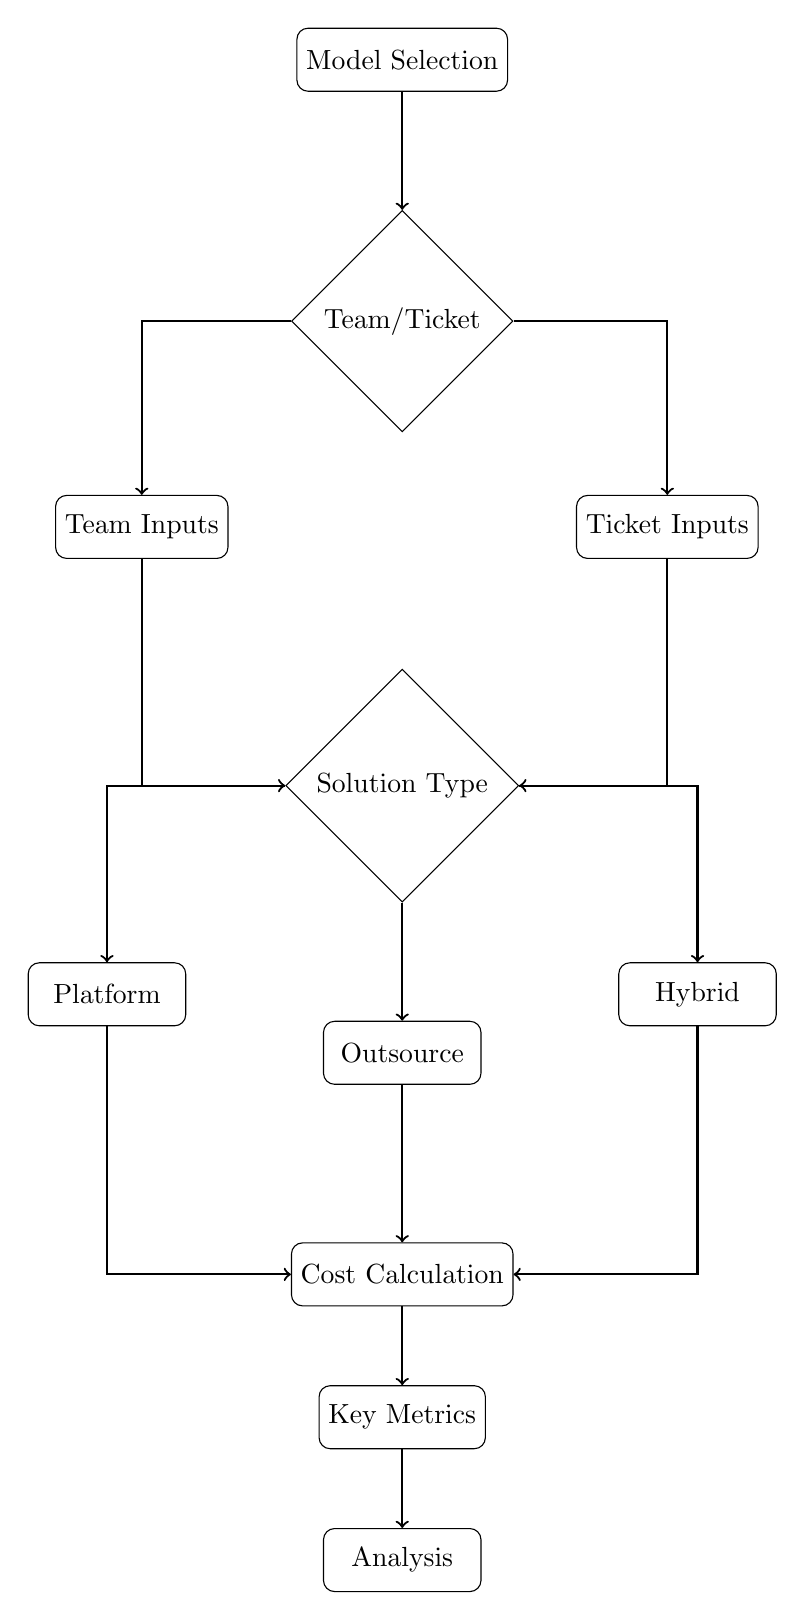
\begin{tikzpicture}[
        node distance=1.5cm,
        block/.style={rectangle, draw=black, fill=white, rounded corners, minimum width=2cm, minimum height=0.8cm},
        process/.style={rectangle, draw=black, fill=white, rounded corners, minimum width=2cm, minimum height=0.8cm}, 
        decision/.style={diamond, draw=black, fill=white, minimum width=2cm, minimum height=0.8cm},
        line/.style={draw, ->, thick}
    ]
        % Input Selection
        \node[block] (model) {Model Selection};
        \node[decision] (type) [below=of model] {Team/Ticket};
        \node[block] (team) [below left=1.5cm and 1.5cm of type] {Team Inputs};
        \node[block] (ticket) [below right=1.5cm and 1.5cm of type] {Ticket Inputs};
        
        % Solution Selection
        \node[decision] (solution) [below=3cm of type] {Solution Type};
        \node[process] (platform) [below left=1.5cm and 2cm of solution] {Platform};
        \node[process] (outsource) [below=1.5cm of solution] {Outsource};
        \node[process] (hybrid) [below right=1.5cm and 2cm of solution] {Hybrid};
        
        % Calculations
        \node[block] (calc) [below=2cm of outsource] {Cost Calculation};
        \node[block] (metrics) [below=1cm of calc] {Key Metrics};
        \node[block] (analysis) [below=1cm of metrics] {Analysis};
        
        % Connections
        \draw[line] (model) -- (type);
        \draw[line] (type) -| (team);
        \draw[line] (type) -| (ticket);
        \draw[line] (team) |- (solution);
        \draw[line] (ticket) |- (solution);
        \draw[line] (solution) -| (platform);
        \draw[line] (solution) -- (outsource);
        \draw[line] (solution) -| (hybrid);
        \draw[line] (platform) |- (calc);
        \draw[line] (outsource) -- (calc);
        \draw[line] (hybrid) |- (calc);
        \draw[line] (calc) -- (metrics);
        \draw[line] (metrics) -- (analysis);
    \end{tikzpicture}
    \caption{Application Implementation Flow}
\end{figure}


\subsection{Team-Based Model Implementation}

\begin{definition}{Base Team Model Inputs}
Required parameters:
\begin{itemize}
    \item \textbf{Team Size (n):} Number of FTEs [1-1000]
    \item \textbf{Hourly Rate (h):} Cost per FTE [\$1-\$1000]
    \item \textbf{Service Delivery ($\eta_s$):} Productive time [0-100\%]
    \item \textbf{Working Hours (w):} Monthly hours [120-200]
    \item \textbf{Overhead ($\eta_o$):} Administrative overhead [0-100\%]
\end{itemize}

Cost calculation:
\begin{equation}
    C_{base} = n \cdot h \cdot w \cdot \eta_s \cdot (1 + \eta_o)
\end{equation}

Key metrics:
\begin{itemize}
    \item \textbf{Monthly Cost:} Direct calculation from formula
    \item \textbf{Team Utilization:} $\eta_s \cdot 100\%$
    \item \textbf{Cost per FTE:} $\frac{C_{base}}{n}$
\end{itemize}
\end{definition}

\begin{definition}{Team Platform Solution Inputs}
Required parameters:
\begin{itemize}
    \item \textbf{Initial Cost ($P_i$):} Platform investment [\$0-\$10M]
    \item \textbf{Build Time ($T_i$):} Implementation period [1-24 months]
    \item \textbf{Maintenance ($P_m$):} Monthly upkeep [\$0-\$1M]
    \item \textbf{Team Reduction ($\alpha_t$):} Staff efficiency [0-100\%]
    \item \textbf{Process Efficiency ($\alpha_p$):} Automation impact [0-100\%]
\end{itemize}

Cost calculation:
\begin{equation}
    C_{platform} = C_{base} \cdot (1 - \alpha_t) \cdot (1 - \alpha_p) + P_m
\end{equation}

Key metrics:
\begin{itemize}
    \item \textbf{Monthly Savings:} $C_{base} - C_{platform}$
    \item \textbf{Break-even Period:} $\frac{P_i}{\text{Monthly Savings}}$
    \item \textbf{ROI:} $\frac{\text{Annual Savings} - P_i}{P_i} \cdot 100\%$
\end{itemize}
\end{definition}

\begin{definition}{Team Outsourcing Solution Inputs}
Required parameters:
\begin{itemize}
    \item \textbf{Vendor Rate (v):} Hourly cost [\$1-\$1000]
    \item \textbf{Transition Time ($T_t$):} Handover period [1-12 months]
    \item \textbf{Transition Cost ($O_t$):} One-time cost [\$0-\$1M]
    \item \textbf{Management Overhead ($\beta_m$):} Additional oversight [0-100\%]
    \item \textbf{Quality Impact ($\beta_q$):} Service degradation [0-100\%]
    \item \textbf{Knowledge Loss ($\beta_k$):} Expertise reduction [0-100\%]
\end{itemize}

Cost calculation:
\begin{equation}
    C_{outsource} = v \cdot w \cdot n \cdot (1 + \beta_m) \cdot (1 + \beta_q) \cdot (1 + \beta_k \cdot \log_{10}(T_t + 1))
\end{equation}

Key metrics:
\begin{itemize}
    \item \textbf{Monthly Savings:} $C_{base} - C_{outsource}$
    \item \textbf{Quality Factor:} $1 - \beta_q$
    \item \textbf{Knowledge Retention:} $1 - \beta_k \cdot \log_{10}(T_t + 1)$
\end{itemize}
\end{definition}

\begin{definition}{Team Hybrid Solution Inputs}
Required parameters:
\begin{itemize}
    \item \textbf{Platform Portion ($\gamma_p$):} Platform coverage [0-100\%]
    \item \textbf{Platform Cost ($P_h$):} Reduced investment [\$0-\$10M]
    \item \textbf{Vendor Portion ($\gamma_o$):} Outsourced portion [0-100\%]
    \item \textbf{Vendor Rate ($v_h$):} Reduced rate [\$1-\$1000]
\end{itemize}

Cost calculation:
\begin{equation}
    C_{hybrid} = \gamma_p \cdot C_{platform} + \gamma_o \cdot C_{outsource}
\end{equation}

Key metrics:
\begin{itemize}
    \item \textbf{Monthly Savings:} $C_{base} - C_{hybrid}$
    \item \textbf{Blended Efficiency:} $\gamma_p \cdot (1 - \alpha_p) + \gamma_o \cdot (1 - \beta_q)$
    \item \textbf{Combined ROI:} $\frac{\text{Annual Savings} - (P_h + O_t)}{P_h + O_t} \cdot 100\%$
\end{itemize}
\end{definition}

\subsection{Ticket-Based Model Implementation}

\begin{definition}{Base Ticket Model Inputs}
Required parameters:
\begin{itemize}
    \item \textbf{Monthly Tickets (m):} Request volume [1-10000]
    \item \textbf{Hours per Ticket ($t_h$):} Resolution time [0.1-100]
    \item \textbf{People per Ticket (p):} Team members needed [1-10]
    \item \textbf{Hourly Rate (h):} Internal cost [\$1-\$1000]
    \item \textbf{SLA Compliance ($\sigma$):} Service level met [0-100\%]
\end{itemize}

Cost calculation:
\begin{equation}
    C_{ticket} = m \cdot t_h \cdot p \cdot h
\end{equation}

Key metrics:
\begin{itemize}
    \item \textbf{Monthly Cost:} Direct calculation from formula
    \item \textbf{Cost per Ticket:} $\frac{C_{ticket}}{m}$
    \item \textbf{Resource Utilization:} $\frac{m \cdot t_h}{w \cdot p} \cdot 100\%$
\end{itemize}
\end{definition}

\begin{definition}{Ticket Platform Solution Inputs}
Required parameters:
\begin{itemize}
    \item \textbf{Initial Cost ($P_i$):} Platform investment [\$0-\$10M]
    \item \textbf{Build Time ($T_i$):} Implementation period [1-24 months]
    \item \textbf{Automation Rate ($\alpha_a$):} Automated tickets [0-100\%]
    \item \textbf{Time Reduction ($\alpha_t$):} Processing speed [0-100\%]
    \item \textbf{Quality Improvement ($\alpha_q$):} Error reduction [0-100\%]
\end{itemize}

Cost calculation:
\begin{equation}
    C_{tp} = m \cdot [\alpha_a \cdot c_a + (1-\alpha_a) \cdot t_h \cdot (1-\alpha_t) \cdot p \cdot h] + P_m
\end{equation}

Key metrics:
\begin{itemize}
    \item \textbf{Automation Rate:} $\alpha_a \cdot 100\%$
    \item \textbf{Processing Efficiency:} $(1 - \alpha_t) \cdot 100\%$
    \item \textbf{Quality Factor:} $1 + \alpha_q$
\end{itemize}
\end{definition}

\begin{definition}{Ticket Outsourcing Solution Inputs}
Required parameters:
\begin{itemize}
    \item \textbf{Ticket Cost ($v_t$):} Cost per ticket [\$1-\$1000]
    \item \textbf{Transition Time ($T_t$):} Handover period [1-12 months]
    \item \textbf{Multiplication Factor ($\mu$):} Volume impact [$\geq 1$]
    \item \textbf{Resolution Factor ($\tau$):} Time impact [$\geq 1$]
    \item \textbf{Rework Rate ($\omega$):} Reopening probability [0-100\%]
\end{itemize}

Cost calculation:
\begin{equation}
    C_{to} = m \cdot v_t \cdot \mu \cdot (1 + \omega) \cdot \tau
\end{equation}

Key metrics:
\begin{itemize}
    \item \textbf{Effective Volume:} $m \cdot \mu \cdot (1 + \omega)$
    \item \textbf{Resolution Rate:} $\frac{1}{\tau}$
    \item \textbf{First Contact Resolution:} $1 - \omega$
\end{itemize}
\end{definition}

\begin{definition}{Ticket Hybrid Solution Inputs}
Required parameters:
\begin{itemize}
    \item \textbf{Automated Portion ($\gamma_a$):} Platform handled [0-100\%]
    \item \textbf{Outsourced Portion ($\gamma_v$):} Vendor handled [0-100\%]
    \item \textbf{Internal Portion ($\gamma_i$):} Manual handled [0-100\%]
    \item \textbf{Automation Success ($\eta_a$):} Platform effectiveness [0-100\%]
\end{itemize}

Cost calculation:
\begin{equation}
    C_{th} = m \cdot (\gamma_a \cdot c_a + \gamma_v \cdot v_t \cdot \mu \cdot \tau + \gamma_i \cdot t_h \cdot p \cdot h)
\end{equation}

Key metrics:
\begin{itemize}
    \item \textbf{Effective Success Rate:} $\gamma_a \cdot \eta_a + \gamma_v \cdot \frac{1}{\mu \cdot \tau} + \gamma_i$
    \item \textbf{Blended Cost per Ticket:} $\frac{C_{th}}{m}$
    \item \textbf{Distribution Balance:} $\gamma_a + \gamma_v + \gamma_i = 1$
\end{itemize}
\end{definition}

\begin{observation}
Implementation considerations:
\begin{itemize}
    \item All inputs require validation within specified ranges
    \item Cost calculations update in real-time as inputs change
    \item Break-even calculations consider initial investments
    \item ROI metrics account for both cost savings and quality impacts
    \item Sensitivity analysis applies ±20\% variation to key parameters
\end{itemize}
\end{observation}

\end{document}